\chapter{样本及抽样分布}

% ============ §1 随机样本 ============
\section{随机样本}

\subsection{总体与样本}

\begin{definition}[总体与个体]
\textbf{总体}（母体）是研究对象的全体，通常用一个随机变量 $X$ 表示，其分布函数为 $F(x)$。
\textbf{个体}是组成总体的每个元素。
\end{definition}

\begin{definition}[简单随机样本]
设 $X$ 是具有分布函数 $F$ 的随机变量，若 $X_1, X_2, \dots, X_n$ 满足：
\begin{enumerate}[label=(\roman*)]
    \item \textbf{代表性}：每个 $X_i$ 与 $X$ 有相同的分布函数 $F$；
    \item \textbf{独立性}：$X_1, X_2, \dots, X_n$ 相互独立，
\end{enumerate}
则称为来自总体 $X$ 的容量为 $n$ 的\textbf{简单随机样本}，简称样本。
记作：
\begin{equation}
    X_1, X_2, \dots, X_n \stackrel{\mathrm{i.i.d.}}{\sim} F(x).
\end{equation}
\end{definition}

当获得一组具体观测值 $x_1, x_2, \dots, x_n$ 时，称其为\textbf{样本值}。

\begin{remark}[总体、个体、样本：用三组例子建立直觉]
\textbf{"总体"不是物理对象的集合，而是你关心的那个\emph{量}在所有个体上的取值及其概率规律。}

\begin{center}
\renewcommand{\arraystretch}{1.3}
\begin{tabular}{c|c|c|c}
\toprule
\textbf{实际问题} & \textbf{总体（随机变量 $X$）} & \textbf{个体} & \textbf{样本（$n$ 个个体的观测值）} \\
\midrule
评估灯泡寿命   & 这批灯泡的寿命值及其分布  & 每只灯泡   & 随机抽 $n$ 只灯泡，测出其寿命 $x_1,\dots,x_n$ \\
了解居民收入   & 某市所有居民的年收入分布    & 每位居民   & 随机调查 $n$ 位居民的年收入 $x_1,\dots,x_n$ \\
监控螺栓直径   & 某产线所有螺栓的直径分布    & 每个螺栓   & 随机抽取 $n$ 个螺栓，测出直径 $x_1,\dots,x_n$ \\
\bottomrule
\end{tabular}
\end{center}

\medskip
\textbf{注意"样本"一词的双重含义：}

\begin{center}
\begin{tabular}{c|c|c}
\toprule
\textbf{语境} & \textbf{含义} & \textbf{记号} \\
\midrule
抽样前（理论上） & $n$ 个随机变量，各与总体同分布且相互独立 & 大写 $X_1,\dots,X_n$ \\
抽样后（实际上） & 做实验得到的 $n$ 个具体数字              & 小写 $x_1,\dots,x_n$ \\
\bottomrule
\end{tabular}
\end{center}

例如 $\bar{X} = \frac{1}{n}\sum X_i$ 是随机变量（统计量），而 $\bar{x} = \frac{1}{n}\sum x_i$ 是一个具体数值。
整个统计推断的逻辑链是：\textbf{用已知的 $\bar{x}$ 去反推未知的 $\mu$，中间桥梁是 $\bar{X}$ 的抽样分布。}
\end{remark}

\begin{remark}["简单随机样本"中"简单"与"随机"的含义]
\textbf{随机} = 抽样时每个个体被选入样本的概率均等，结果由概率决定而非人为挑选。

\textbf{简单} = 满足两个条件：
\begin{enumerate}[label=(\roman*)]
    \item \textbf{代表性（同分布）}：每个 $X_i$ 与总体 $X$ 的波动规律完全相同。\\
    反例——第 1 个灯泡来自 A 厂、第 2 个来自不相关的 B 厂，两者分布不同，不满足同分布。
    \item \textbf{独立性}：知道 $X_1$ 的取值不能提供任何关于 $X_2$ 的信息。\\
    反例——不放回抽样在有限总体中严格不独立，但当总体容量 $\gg n$ 时可近似视为独立。
\end{enumerate}

两者本质上等价于 $X_1,\dots,X_n \stackrel{\mathrm{i.i.d.}}{\sim} F(x)$（独立同分布样本）。

\medskip
\textbf{一句话区分：}
\begin{center}
\begin{tabular}{c|c}
\toprule
\textbf{术语} & \textbf{回答的问题} \\
\midrule
随机 & 谁被选入样本？——由概率决定，非人为挑选 \\
简单 & 入选个体的数据有何规律？——彼此独立、同分布 \\
\bottomrule
\end{tabular}
\end{center}
\end{remark}

\subsubsection{从总体到统计量：四步概念梳理}

以下用四步串联"总体 → 样本 → 统计量"的逻辑链条，并指出常见误区。

\begin{enumerate}[label=\textbf{第 \arabic* 步}, leftmargin=*]

    \item \textbf{从总体中抽取一个容量为 $n$ 的样本。}

    \emph{常见误区：} "抽样 $n$ 次"听起来像做了 $n$ 轮独立实验，容易和重复抽样混淆。
    正确说法是：从总体 $X$ 中\emph{一次性}抽取 $n$ 个独立同分布的个体，
    记作 $X_1, X_2, \dots, X_n \stackrel{\mathrm{i.i.d.}}{\sim} F(x)$。

    \item \textbf{每个 $X_i$ 是独立同分布随机变量，但分布参数 $\mu, \sigma^2$ 未知。}

    在\emph{参数统计}中，通常假设已知分布的形式（如正态），仅参数未知：
    \begin{center}
    \begin{tabular}{c|c}
    \toprule
    已知 & 未知 \\
    \midrule
    $X_i \sim \mathcal{N}(\mu, \sigma^2)$（分布族） & $\mu$ 和 $\sigma^2$ 的具体值 \\
    $X_i \sim \mathrm{Bernoulli}(p)$               & $p$ 的具体值 \\
    \bottomrule
    \end{tabular}
    \end{center}

    如果连分布形式都不知道，那属于\emph{非参数统计}的范畴。后续所有内容
    （MLE、$t$ 检验、置信区间）均建立在"已知分布族，未知参数"的前提下。

    \textbf{关键区分：}$\mu$ 和 $\sigma^2$ 是\emph{总体的}均值和方差（固定但未知的常数）；
    $\bar{X}$ 和 $S^2$ 是\emph{样本的}均值和方差（随机变量，用来估计它们）。

    \item \textbf{定义样本均值 $\bar{X}$ —— 第一个核心统计量。}

    \begin{equation}
        \bar{X} = \frac{1}{n} \sum_{i=1}^{n} X_i
    \end{equation}

    注意：不是 $\hat{-}X$！标准写法是 $\bar{X}$（\verb|\bar{X}|），读作"X bar"。

    $\bar{X}$ 有两个身份：
    \begin{itemize}
        \item \textbf{统计量}：抽样前是随机变量，有自己的分布 $\bar{X} \sim \mathcal{N}(\mu, \sigma^2/n)$
        \item \textbf{估计量}：用来估计总体均值 $\mu$，且是无偏的（$\E[\bar{X}] = \mu$）
    \end{itemize}

    这里没有"组"的概念——"组内均值"是 ANOVA 里的术语（多组比较时组内 vs. 组间）。
    在单样本场景下，它就是\emph{样本均值}。

    \item \textbf{定义样本方差 $S^2$ —— 第二个核心统计量。}

    \begin{equation}
        S^2 = \frac{1}{n-1} \sum_{i=1}^{n} (X_i - \bar{X})^2
    \end{equation}

    用于刻画样本内部的离散程度（而非"组内差异"），同时也是总体方差 $\sigma^2$ 的无偏估计量。
    分母 $n-1$ 的来源已在上一节完整推导。

\end{enumerate}

\textbf{四步总览：}

\begin{center}
\fbox{%
\begin{minipage}{0.88\textwidth}
\[
\text{总体 } X \sim F(x;\theta),\ \mu,\sigma^2 \text{ 未知}
\quad\xrightarrow{\text{抽取 } n \text{ 个 i.i.d. 个体}}\quad
\underbrace{X_1,\dots,X_n}_{\text{样本（随机变量）}}
\quad\xrightarrow{\text{构造统计量}}\quad
\begin{cases}
\bar{X} = \frac{1}{n}\sum X_i          & \to \text{估计 } \mu \\[6pt]
S^2 = \frac{1}{n-1}\sum (X_i - \bar{X})^2 & \to \text{估计 } \sigma^2
\end{cases}
\]
\end{minipage}}
\end{center}

整个数理统计的核心任务就是：\textbf{用已知的 $\bar{x}$ 和 $s^2$（观测值）反推未知的 $\mu$ 和 $\sigma^2$（总体参数），
而反推的依据就是 $\bar{X}$ 和 $S^2$ 的抽样分布。}

\begin{definition}[统计量]
设 $X_1, \dots, X_n$ 是来自总体 $X$ 的样本，$g(x_1, \dots, x_n)$ 是\textbf{不含任何未知参数}的函数，则称
\begin{equation}
    T = g(X_1, X_2, \dots, X_n)
\end{equation}
为一个\textbf{统计量}。统计量是随机变量的函数，因此它本身也是一个随机变量。
\end{definition}

\subsection{常用统计量}

\begin{definition}[样本均值]
\begin{equation}
    \bar{X} = \frac{1}{n} \sum_{i=1}^{n} X_i.
\end{equation}
\end{definition}

\begin{definition}[样本方差与样本标准差]
\begin{align}
    S^2     &= \frac{1}{n-1} \sum_{i=1}^{n} (X_i - \bar{X})^2, \\
    S       &= \sqrt{S^2}.
\end{align}
\textbf{为什么分母是 $n-1$？——完整推导}
\end{definition}

\subsubsection{推导目标}

证明：若用 $n-1$ 作分母，则 $\E[S^2] = \sigma^2$（无偏）；若用 $n$ 作分母，则估计有偏。

\subsubsection{前提假设}

设总体 $X$ 的均值 $\E[X] = \mu$，方差 $\Var(X) = \sigma^2$。
$X_1, X_2, \dots, X_n \stackrel{\mathrm{i.i.d.}}{\sim} X$，样本均值 $\bar{X} = \frac{1}{n}\sum_{i=1}^{n} X_i$。

\subsubsection{关键恒等式}

\begin{equation}
    \sum_{i=1}^{n} (X_i - \bar{X})^2 = \sum_{i=1}^{n} X_i^2 - n\bar{X}^2.
    \label{eq:key-identity}
\end{equation}

\textbf{验证：}
\begin{align}
    \sum_{i=1}^{n} (X_i - \bar{X})^2
    &= \sum_{i=1}^{n} \big(X_i^2 - 2X_i\bar{X} + \bar{X}^2\big)
     = \sum_{i=1}^{n} X_i^2 - 2\bar{X}\underbrace{\sum_{i=1}^{n} X_i}_{= n\bar{X}} + n\bar{X}^2 \nonumber\\
    &= \sum_{i=1}^{n} X_i^2 - 2n\bar{X}^2 + n\bar{X}^2
     = \sum_{i=1}^{n} X_i^2 - n\bar{X}^2. \nonumber
\end{align}

\subsubsection{逐项求期望}

\textbf{第一项：} $\E\!\left[\sum X_i^2\right]$

对每个 $X_i$，由 $\Var(X_i) = \E[X_i^2] - (\E[X_i])^2$，得：
\begin{equation}
    \E[X_i^2] = \Var(X_i) + (\E[X_i])^2 = \sigma^2 + \mu^2.
\end{equation}
由于 $n$ 个变量同分布：
\begin{equation}
    \E\!\left[\sum_{i=1}^{n} X_i^2\right] = \sum_{i=1}^{n} \E[X_i^2]
    = n(\sigma^2 + \mu^2).
    \label{eq:term1}
\end{equation}

\textbf{第二项：} $\E\!\left[n\bar{X}^2\right]$

先求 $\bar{X}$ 的期望与方差：
\begin{align}
    \E[\bar{X}]   &= \E\!\left[\frac{1}{n}\sum X_i\right] = \frac{1}{n}\sum \E[X_i] = \mu, \\
    \Var(\bar{X}) &= \Var\!\left(\frac{1}{n}\sum X_i\right)
                    = \frac{1}{n^2}\sum \Var(X_i) \quad \text{(独立性)}
                    = \frac{1}{n^2} \cdot n\sigma^2 = \frac{\sigma^2}{n}.
\end{align}

于是：
\begin{equation}
    \E[\bar{X}^2] = \Var(\bar{X}) + (\E[\bar{X}])^2 = \frac{\sigma^2}{n} + \mu^2.
\end{equation}

因此：
\begin{equation}
    \E\!\left[n\bar{X}^2\right] = n \cdot \E[\bar{X}^2]
    = n\left(\frac{\sigma^2}{n} + \mu^2\right)
    = \sigma^2 + n\mu^2.
    \label{eq:term2}
\end{equation}

\subsubsection{合并得到最终结果}

将式 $(\ref{eq:term1})$ 与 $(\ref{eq:term2})$ 代入恒等式 $(\ref{eq:key-identity})$ 的期望：
\begin{align}
    \E\!\left[\sum_{i=1}^{n} (X_i - \bar{X})^2\right]
    &= \E\!\left[\sum_{i=1}^{n} X_i^2\right] - \E\!\left[n\bar{X}^2\right] \nonumber\\
    &= n(\sigma^2 + \mu^2) - (\sigma^2 + n\mu^2) \nonumber\\
    &= (n-1)\sigma^2.
    \label{eq:final-expectation}
\end{align}

\subsubsection{结论}

\begin{definition}[无偏样本方差]
由式 $(\ref{eq:final-expectation})$，定义：
\begin{equation}
    \boxed{S^2 = \frac{1}{n-1} \sum_{i=1}^{n} (X_i - \bar{X})^2},
\end{equation}
则有：
\begin{equation}
    \boxed{\E[S^2] = \frac{1}{n-1} \cdot (n-1)\sigma^2 = \sigma^2}.
\end{equation}
即 $S^2$ 是总体方差 $\sigma^2$ 的\textbf{无偏估计量}。
\end{definition}

\begin{remark}[若用 $n$ 作分母]
定义有偏版本 $\tilde{S}^2 = \frac{1}{n}\sum_{i=1}^{n} (X_i - \bar{X})^2 = B_2$（二阶中心矩），则：
\begin{equation}
    \E[\tilde{S}^2] = \frac{n-1}{n}\,\sigma^2 < \sigma^2 \quad (n \ge 2).
\end{equation}
它\textbf{系统性地低估}总体方差。当 $n \to \infty$ 时 $\frac{n-1}{n} \to 1$，故 $\tilde{S}^2$ 是\textbf{渐近无偏}的。
\end{remark}

\subsubsection{直观解释：自由度的损失}

为什么"丢失"了 1？因为我们在计算 $\bar{X}$ 时用掉了数据的一个线性关系：
\begin{equation}
    \sum_{i=1}^{n} (X_i - \bar{X}) = 0.
\end{equation}
这个约束意味着 $n$ 个偏差 $(X_i - \bar{X})$ 中只有 $n-1$ 个是可以自由变化的。因此\textbf{自由度}为 $n-1$，除以 $n-1$ 才能得到无偏估计。

可以这样记忆：
\begin{itemize}
    \item $\bar{X}$ 是 $\mu$ 的无偏估计，分母用 $n$（自由度 = $n$）
    \item $S^2$ 是 $\sigma^2$ 的无偏估计，分母用 $n-1$（自由度 = $n-1$，因为用 $\bar{X}$ 替代了 $\mu$）
\end{itemize}

\begin{definition}[样本 $k$ 阶原点矩与中心矩]
\begin{align}
    A_k &= \frac{1}{n} \sum_{i=1}^{n} X_i^k \quad \text{($k$ 阶原点矩)}, \\
    B_k &= \frac{1}{n} \sum_{i=1}^{n} (X_i - \bar{X})^k \quad \text{($k$ 阶中心矩)}.
\end{align}
\end{definition}

\begin{definition}[次序统计量]
将样本观测值从小到大排序：$x_{(1)} \le x_{(2)} \le \dots \le x_{(n)}$，对应的随机变量
$X_{(1)}, X_{(2)}, \dots, X_{(n)}$ 称为\textbf{次序统计量}。
\begin{itemize}
    \item $X_{(1)} = \min\{X_1,\dots,X_n\}$ — 最小次序统计量
    \item $X_{(n)} = \max\{X_1,\dots,X_n\}$ — 最大次序统计量
    \item 样本中位数 $M_e$，样本极差 $R = X_{(n)} - X_{(1)}$
\end{itemize}
\end{definition}

% ============ §2 直方图和箱线图 ============
\section{直方图和箱线图}

\subsection{直方图}

\textbf{绘制步骤：}
\begin{enumerate}
    \item 将数据范围分成若干等宽区间（组距）；
    \item 统计落入每个区间的数据个数（频数）或比例（频率）；
    \item 以区间为底、频数/频率为高画矩形。
\end{enumerate}

\textbf{作用：} 观察数据分布的形态——对称性、偏态、峰度、是否多峰、是否有离群值。

\subsection{箱线图}

\textbf{五数概括：}
\begin{itemize}
    \item 最小值 $x_{\min}$（或下须线端点）
    \item 第一四分位数 $Q_1$（第 25 百分位数）
    \item 中位数 $M_e$（第 50 百分位数）
    \item 第三四分位数 $Q_3$（第 75 百分位数）
    \item 最大值 $x_{\max}$（或上须线端点）
\end{itemize}

\textbf{四分位距：}
\begin{equation}
    \mathrm{IQR} = Q_3 - Q_1.
\end{equation}

\textbf{异常值检测：} 小于 $Q_1 - 1.5 \times \mathrm{IQR}$ 或大于 $Q_3 + 1.5 \times \mathrm{IQR}$ 的值视为异常值。

\subsubsection{箱线图结构示意}

\begin{figure}[htbp]
\centering
\begin{tikzpicture}[
    scale=0.6,
    box/.style={very thick, draw=blue!60!black},
    median/.style={very thick, draw=red!70!black},
    whisker/.style={thick, draw=blue!40!black},
    fence/.style={densely dashed, draw=gray, thin},
    annot/.style={font=\scriptsize\sffamily},
    outlier/.style={draw=red!80!black, fill=red!30, circle, inner sep=1.2pt},
]

% ---- 坐标设定 ----
\def\Qone{4}
\def\Med{6.5}
\def\Qthree{9}
\def\LowerWhisker{2}
\def\UpperWhisker{12}

% ---- 坐标轴 ----
\draw[->, thick] (-1, 0) -- (18, 0) node[right] {$x$};
\foreach \x in {0,2,4,6,8,10,12,14,16} {
    \draw (\x, -0.12) -- (\x, 0.12);
    \node[annot, below] at (\x, -0.12) {\x};
}

% ---- 箱体 ----
\fill[blue!8]  (\Qone, 0.6) rectangle (\Qthree, 1.8);
\draw[box]     (\Qone, 0.6) rectangle (\Qthree, 1.8);

% ---- 中位线 ----
\draw[median] (\Med, 0.6) -- (\Med, 1.8);

% ---- 须线 ----
\draw[whisker] (\LowerWhisker, 1.2) -- (\Qone, 1.2);
\draw[whisker] (\LowerWhisker, 0.8) -- (\LowerWhisker, 1.6);
\draw[whisker] (\Qthree, 1.2) -- (\UpperWhisker, 1.2);
\draw[whisker] (\UpperWhisker, 0.8) -- (\UpperWhisker, 1.6);

% ---- 内限虚线 ----
\draw[fence] (-3.5, 0.2) -- (-3.5, 2.2);
\draw[fence] (16.5, 0.2) -- (16.5, 2.2);

% ---- 异常值 ----
\node[outlier] at (0.5, 1.2) {};
\node[outlier] at (15, 1.2) {};

% ===== 标注 =====

% 下方：Q1, Q3, IQR, fence
\draw[annot, <->, >=stealth] (\Qone, -0.5)  -- node[below, fill=white] {$Q_1$} (\Qone, -0.5);
\draw[annot, <->, >=stealth] (\Qthree, -0.5)-- node[below, fill=white] {$Q_3$} (\Qthree, -0.5);
\draw[annot, <->, >=stealth, blue!60!black] (\Qone, 0.35) -- node[below, fill=white, blue!60!black] {\small IQR} (\Qthree, 0.35);
\node[annot, gray] at (-3.5, -0.35) {$Q_1-1.5\mathrm{IQR}$};
\node[annot, gray] at (16.5, -0.35) {$Q_3+1.5\mathrm{IQR}$};

% 中位数
\node[annot, above] at (\Med, 1.95) {$M_e$};

% 异常值标签（紧凑）
\node[annot, red!80!black] at (0.5, 0.95)  {\small 离群点};
\node[annot, red!80!black] at (15,  0.95)  {\small 离群点};

% 须线标签
\node[annot, blue!40!black] at (1.0, 1.55)  {\small 下须线};
\node[annot, blue!40!black] at (13.5,1.55)  {\small 上须线};

% ---- 图例 ----
\node[draw, rounded corners, anchor=north east, font=\scriptsize\sffamily, align=left,
      fill=white, inner sep=4pt] at (17.5, 2.8) {
    须线端点: $\min\{x_i \mid x_i \ge Q_1-1.5\mathrm{IQR}\}$ \\
    \hspace{4.8em} 或 $\max\{x_i \mid x_i \le Q_3+1.5\mathrm{IQR}\}$ \\
    虚线: 内限 (fence)，之外为异常值
};

\end{tikzpicture}
\caption{箱线图结构示意。箱体范围从 $Q_1$ 到 $Q_3$，箱内红线为中位数 $M_e$。须线延伸至非异常值的最远端。
虚线的内限（fence，$Q_1 \pm 1.5\times\mathrm{IQR}$）之外的点为异常值/离群点（红色圆点）。}
\label{fig:boxplot}
\end{figure}

\subsubsection{异常值判定规则}

\begin{center}
\begin{tabular}{c|c|c}
\toprule
\textbf{条件} & \textbf{判定} & \textbf{标记方式} \\
\midrule
$Q_1 - 3\times\mathrm{IQR} \le x_i < Q_1 - 1.5\times\mathrm{IQR}$ & 温和异常值 & \tikz \fill[red!30, draw=red!80!black] (0,0) circle (2pt); \\
$x_i < Q_1 - 3\times\mathrm{IQR}$ & 极端异常值 & \tikz \fill[red!60, draw=red!90!black] (0,0) circle (2pt); （或 $\star$）\\
$Q_3 + 1.5\times\mathrm{IQR} < x_i \le Q_3 + 3\times\mathrm{IQR}$ & 温和异常值 & \tikz \fill[red!30, draw=red!80!black] (0,0) circle (2pt); \\
$x_i > Q_3 + 3\times\mathrm{IQR}$ & 极端异常值 & \tikz \fill[red!60, draw=red!90!black] (0,0) circle (2pt); \\
\bottomrule
\end{tabular}
\end{center}

\subsection{经验分布函数}

\begin{definition}[经验分布函数]
设样本观测值为 $x_1, \dots, x_n$，经验分布函数定义为：
\begin{equation}
    F_n(x) = \frac{1}{n} \sum_{i=1}^{n} \mathbf{1}_{\{x_i \le x\}}
    = \frac{\#\{i: x_i \le x\}}{n}.
\end{equation}
由格里汶科定理，$n \to \infty$ 时 $F_n(x)$ 一致收敛于总体分布 $F(x)$。
\end{definition}

% ============ §3 抽样分布 ============
\section{抽样分布}

统计量的分布称为\textbf{抽样分布}。下面介绍三大重要抽样分布。

\subsection{$\chi^2$ 分布（卡方分布）}

\subsubsection{历史背景}

1900 年，英国统计学家 \textbf{Karl Pearson}（卡尔·皮尔逊）在研究分类数据的拟合优度时，发现了一个核心问题：
掷骰子 60 次，各面分别出现 10, 8, 12, 9, 11, 10 次——这是正常的随机波动，还是骰子有问题？
他把观测频数与期望频数的偏差平方除期望频数后求和，发现这个统计量在大样本下服从一个特定分布，
他将其称为 $\chi^2$ 分布。这篇论文标志着现代假设检验的诞生。

\textbf{为什么叫"卡方"？} $\chi$ 是希腊字母 chi（读作"卡"），$\chi^2$ 就是"chi 的平方"。
它本质上是 $n$ 个独立标准正态随机变量的平方和。

\subsubsection{直观理解}

想象你从 $\mathcal{N}(0,1)$ 中独立抽取 $n$ 个值 $Z_1, \dots, Z_n$：
\begin{itemize}
    \item 每个 $Z_i^2$ 都是非负的，大多数在 $0$ 到 $1$ 之间（因为 $P(|Z|<1) \approx 68\%$）
    \item 把 $n$ 个这样的非负数加起来，总和大概在 $n$ 附近——这就是 $\E[\chi^2] = n$ 的直觉
    \item $n$ 越大，求和的结果波动越大——$\Var(\chi^2) = 2n$ 反映了这一点
\end{itemize}

自由度 $n$ = 独立信息的个数。每用掉一个估计量（如用 $\bar{X}$ 替代 $\mu$），自由度减 1。

\subsubsection{核心问题：总体不是 $\mathcal{N}(0,1)$ 时怎么用卡方？}

\emph{这是初学者最困惑的地方。} $\chi^2$ 分布的定义要求 $X_i \sim \mathcal{N}(0,1)$，
但在实际中你只知道 $X_i \sim \mathcal{N}(\mu, \sigma^2)$，$\mu$ 和 $\sigma^2$ 都未知。
\textbf{怎么把一般的正态样本转化为卡方变量？}

\medskip
\textbf{完整推导流程（三步桥接）：}

\begin{enumerate}[label=\textbf{第 \arabic* 步}, leftmargin=*]

    \item \textbf{先假设 $\mu$ 已知 —— 标准化。}

    若 $\mu$ 已知，对每个 $X_i$ 做标准化：
    \begin{equation}
        Z_i = \frac{X_i - \mu}{\sigma} \sim \mathcal{N}(0,1).
    \end{equation}

    那么 $n$ 个 $Z_i$ 的平方和就是卡方：
    \begin{equation}
        \sum_{i=1}^{n} Z_i^2 = \sum_{i=1}^{n} \left(\frac{X_i - \mu}{\sigma}\right)^2 \sim \chi^2(n).
        \label{eq:chi2-if-mu-known}
    \end{equation}

    自由度是 $n$，因为 $n$ 个 $X_i$ 提供了 $n$ 个独立信息，没有被消耗的。

    \item \textbf{现实中 $\mu$ 未知 —— 用 $\bar{X}$ 替代 $\mu$，自由度减 1。}

    实际中 $\mu$ 未知，你只能用 $\bar{X}$ 来替代它：
    \begin{equation}
        \sum_{i=1}^{n} \left(\frac{X_i - \textcolor{red}{\bar{X}}}{\sigma}\right)^2
        = \frac{1}{\sigma^2} \sum_{i=1}^{n} (X_i - \bar{X})^2.
    \end{equation}

    这个量还是卡方吗？\textbf{是的，但自由度减少了 1：}
    \begin{equation}
        \boxed{\frac{\sum_{i=1}^{n} (X_i - \bar{X})^2}{\sigma^2} \sim \chi^2(n-1)}.
        \label{eq:chi2-key}
    \end{equation}

    \textbf{为什么自由度从 $n$ 变成 $n-1$？}

    因为 $\bar{X}$ 是从数据本身估计出来的，这引入了一个约束：
    $\sum_{i=1}^{n} (X_i - \bar{X}) = 0$。
    $n$ 个偏差中只有 $n-1$ 个可以自由变化，最后一个被前 $n-1$ 个决定。
    每消耗一个估计量（用 $\bar{X}$ 替代 $\mu$），自由度就减 1。
    这就和之前推导 $S^2$ 时 $\E[S^2] = \sigma^2$（分母 $n-1$）是同一个逻辑。

    \item \textbf{等价形式 —— 用样本方差 $S^2$ 表达。}

    由 $S^2 = \frac{1}{n-1}\sum (X_i - \bar{X})^2$，式 $(\ref{eq:chi2-key})$ 等价于：
    \begin{equation}
        \boxed{\frac{(n-1)S^2}{\sigma^2} \sim \chi^2(n-1)}.
        \label{eq:chi2-sample-var}
    \end{equation}

    这是\emph{最常用的形式}，因为 $S^2$ 可以直接从样本算出来。
\end{enumerate}

\medskip
\textbf{完整数值示例：}

假设某工厂螺栓直径服从 $\mathcal{N}(\mu, \sigma^2)$，$\mu$ 和 $\sigma^2$ 均未知。
抽取 $n = 10$ 个螺栓，测得样本方差 $s^2 = 0.04$。

\begin{itemize}
    \item 若想知道 $\sigma^2$ 是否等于某标称值 $\sigma_0^2 = 0.02$：
    \item 计算检验统计量：$\dfrac{(n-1)s^2}{\sigma_0^2} = \dfrac{9 \times 0.04}{0.02} = 18$
    \item 在原假设 $H_0: \sigma^2 = 0.02$ 下，该统计量 $\sim \chi^2(9)$
    \item 查表：$\chi^2_{0.05}(9) \approx 16.92$，$18 > 16.92$，拒绝 $H_0$，认为实际方差偏大
\end{itemize}

\medskip
\textbf{一句话总结：}

\[
\text{$\chi^2$ 定义要求的标准正态 } \xrightarrow{\text{标准化 } Z_i = \frac{X_i - \mu}{\sigma}}
\text{ 一般正态样本 } \xrightarrow{\text{$\mu$ 未知，用 $\bar{X}$ 替代}}
\frac{(n-1)S^2}{\sigma^2} \sim \chi^2(n-1)
\]

\subsubsection{典型应用场景}

\begin{enumerate}[label=(\arabic*)]
    \item \textbf{方差估计与检验}：$\dfrac{(n-1)S^2}{\sigma^2} \sim \chi^2(n-1)$，用于构造 $\sigma^2$ 的置信区间和检验 $H_0: \sigma^2 = \sigma_0^2$（已在上节详述）
    \item \textbf{拟合优度检验（Pearson $\chi^2$ 检验）}：检验观测数据是否符合某个理论分布
    \item \textbf{独立性检验（列联表）}：检验两个分类变量是否独立
    \item \textbf{机器学习中的特征选择}：$\chi^2$ 检验用于评估分类特征与标签之间的相关性
\end{enumerate}

\subsubsection{拟合优度检验——完整流程与实例}

\textbf{问题：} 骰子是否均匀？掷 60 次，观测到各面出现的次数为：

\begin{center}
\begin{tabular}{c|cccccc|c}
\toprule
骰子面 & 1 & 2 & 3 & 4 & 5 & 6 & 合计 \\
\midrule
观测频数 $O_i$ & 7 & 12 & 9 & 13 & 8 & 11 & 60 \\
\bottomrule
\end{tabular}
\end{center}

\textbf{第 1 步：建立假设。}

\begin{itemize}
    \item $H_0$：骰子是均匀的（每一面出现的概率 $p_i = \frac{1}{6}$）
    \item $H_1$：骰子不均匀（至少有一面概率 $\neq \frac{1}{6}$）
\end{itemize}

\textbf{第 2 步：计算期望频数 $E_i$。}

在 $H_0$ 成立的前提下，每一面的期望频数 = $n \times p_i = 60 \times \frac{1}{6} = 10$。

\begin{center}
\begin{tabular}{c|cccccc}
\toprule
骰子面 & 1 & 2 & 3 & 4 & 5 & 6 \\
\midrule
期望频数 $E_i$ & 10 & 10 & 10 & 10 & 10 & 10 \\
\bottomrule
\end{tabular}
\end{center}

\textbf{第 3 步：计算 Pearson $\chi^2$ 统计量。}

\begin{equation}
    \chi^2 = \sum_{i=1}^{k} \frac{(O_i - E_i)^2}{E_i}.
\end{equation}

\textbf{核心直觉：} 分子 $(O_i - E_i)^2$ 度量"观测与期望偏离了多少"；
分母 $E_i$ 做归一化（$E_i$ 大的类别允许更大的绝对偏差）。

逐项计算：
\begin{align}
    \frac{(7-10)^2}{10} + \frac{(12-10)^2}{10} + \frac{(9-10)^2}{10}
    + \frac{(13-10)^2}{10} + \frac{(8-10)^2}{10} + \frac{(11-10)^2}{10}
    &= \frac{9+4+1+9+4+1}{10} \\
    &= 2.8.
\end{align}

\textbf{第 4 步：确定自由度，查临界值。}

\begin{itemize}
    \item $k = 6$ 个类别
    \item 没有从数据中估计任何参数（$m = 0$，概率 $p_i$ 完全由 $H_0$ 指定，而非从样本估计）
    \item 约束：$\sum O_i = n$（每个观测值贡献独立信息，但总和固定），消耗 1 个自由度
    \item 自由度：$df = k - 1 - m = 6 - 1 - 0 = 5$
\end{itemize}

在大样本下，$\chi^2 = 2.8 \sim \chi^2(5)$。取 $\alpha = 0.05$，查表得 $\chi^2_{0.05}(5) \approx 11.07$。

\textbf{第 5 步：做结论。}

$2.8 < 11.07$，统计量不在拒绝域内，不能拒绝 $H_0$——现有数据不足以认为骰子不均匀。

\medskip
\textbf{自由度公式解释：}$df = k - 1 - m$

\begin{itemize}
    \item $k$：类别数
    \item $-1$：因为 $\sum O_i = n$ 是一个固定约束（给定总数后，$k$ 个类别中只有 $k-1$ 个可自由变化）
    \item $-m$：如果 $H_0$ 中的分布参数不是预先指定的，而是先用样本估计的，每估计一个参数再减 1 个自由度。\\
    例：若检验"数据是否服从正态分布"但 $\mu, \sigma^2$ 都需从样本估计，则 $m = 2$，$df = k - 1 - 2$
\end{itemize}

\subsubsection{概念澄清：常见用词误区}

以下用上述"掷骰子"例子对照，纠正初学者在描述流程时常犯的用词错误。

\begin{center}
\footnotesize
\renewcommand{\arraystretch}{1.4}
\begin{tabular}{p{3.2cm}|p{3.8cm}|p{5.5cm}}
\toprule
\textbf{易错表述} & \textbf{问题} & \textbf{正确表述} \\
\midrule
"从认为的概率推出统计量" & 期望频数 $E_i$ \emph{不是}统计量！统计量是从\emph{样本}算出的随机变量
    & $E_i = n \times p_i^{(0)}$ 是 $H_0$ 的推演结果（确定值）；$\chi^2 = \sum (O_i-E_i)^2/E_i$ 才是检验统计量 \\
\midrule
"对两组统计结果进行处理" & 不是"两组数据"！是\emph{同一批样本}的两套频数
    & 观测频数 $O_i$ vs.\ $H_0$ 下的期望频数 $E_i$ \\
\midrule
"用卡方进行检验" & 不是直接用卡方分布去"测"
    & 构造 Pearson $\chi^2$ 统计量，利用其\emph{在 $H_0$ 下的渐近分布}做决策 \\
\bottomrule
\end{tabular}
\end{center}

\medskip
\textbf{修正后的五步标准流程：}

\begin{enumerate}[label=\textbf{第 \arabic* 步}, leftmargin=*]
    \item \textbf{提出 $H_0$}：数据来自某个已知分布（如每面概率 $p_i = 1/6$）。
    \item \textbf{计算期望频数} $E_i = n \times p_i^{(0)}$——这是确定性的数值，\emph{不是统计量}。
    \item \textbf{构造检验统计量} $\chi^2 = \sum \frac{(O_i - E_i)^2}{E_i}$——这才是从样本算出的\emph{统计量}。
    \item \textbf{确定自由度} $df = k - 1 - m$，查 $\chi^2$ 临界值。
    \item \textbf{比较并做结论}：若 $\chi^2 > \chi^2_{\alpha}(df)$，拒绝 $H_0$。
\end{enumerate}

\subsubsection{核心原理：为什么 $\sum (O_i-E_i)^2/E_i$ 服从 $\chi^2$ 分布？}

这是 Pearson 在 1900 年做出的最深洞察。以下分三步推导。

\medskip
\textbf{第 1 步：每个格子的 $O_i$ 本质上是什么？}

$O_i$ 是 $n$ 个独立个体中落入第 $i$ 类的个数。在 $H_0$ 下，每个个体以概率 $p_i$ 落入第 $i$ 类。因此：

\begin{equation}
    O_i \sim \mathrm{Binomial}(n, p_i), \quad
    \E[O_i] = np_i = E_i, \quad
    \Var(O_i) = np_i(1-p_i).
\end{equation}

\medskip
\textbf{第 2 步：标准化 —— 从二项到近似标准正态。}

由中心极限定理（$n$ 大时二项分布近似正态）：

\begin{equation}
    \frac{O_i - E_i}{\sqrt{np_i(1-p_i)}} \xrightarrow{d} \mathcal{N}(0,1).
\end{equation}

在实际应用中，大多数 $p_i$ 不大，$1-p_i \approx 1$，分母可近似为 $\sqrt{np_i} = \sqrt{E_i}$：

\begin{equation}
    \boxed{\frac{O_i - E_i}{\sqrt{E_i}} \;\approx\; \mathcal{N}(0,1)}.
\end{equation}

这一项就是第 $i$ 类的\textbf{标准化偏差}——"观测值偏离了期望值几个标准差"。

\medskip
\textbf{第 3 步：平方求和 —— 从正态到卡方。}

$\chi^2$ 分布的定义就是 $k$ 个独立标准正态的平方和。因此：

\begin{equation}
    \boxed{\chi^2 = \sum_{i=1}^{k} \left(\frac{O_i - E_i}{\sqrt{E_i}}\right)^2
                 = \sum_{i=1}^{k} \frac{(O_i - E_i)^2}{E_i}
                 \;\sim\; \chi^2(k-1)}.
\end{equation}

\textbf{为什么自由度是 $k-1$ 而非 $k$？}

因为 $\sum_{i=1}^{k} O_i = n$ 是一个固定约束——$k$ 个偏差中只有 $k-1$ 个可以独立变化，最后一个被前 $k-1$ 个自动决定。
（若 $H_0$ 中有 $m$ 个参数是用样本估计的，则再减 $m$。）

\medskip
\textbf{一句话直觉：}

\[
\frac{O_i - E_i}{\sqrt{E_i}}
\;\underbrace{\longrightarrow}_{\text{平方}}\;
\frac{(O_i - E_i)^2}{E_i}
\;\underbrace{\longrightarrow}_{\text{对所有 $k$ 类求和}}\;
\chi^2
\;\underbrace{\longrightarrow}_{\text{查表}}\;
\text{判断是否显著偏离 } H_0
\]

\begin{itemize}
    \item 若 $H_0$ 为真，每个 $\frac{O_i - E_i}{\sqrt{E_i}}$ 大约在 $\pm 1$ 范围内，平方后 $\approx 1$，总和 $\approx k-1$（即期望值 = 自由度）
    \item 若 $H_0$ 为假，某些类别的偏差远大于 $1$ 个标准差，平方后急剧放大，总和 $\gg k-1$，落入拒绝域
\end{itemize}

这就是为什么\textbf{这个看似简单的公式能区分"随机波动"和"真正的分布差异"}——它在数学上等价于把每个类别的标准化偏差平方后累加，然后用卡方分布精确量化"这么大的总和由纯随机产生的概率有多大"。

\textbf{问题：} 性别与是否吸烟是否独立？调查 200 人，得到以下 $2 \times 2$ 列联表：

\begin{center}
\begin{tabular}{c|cc|c}
\toprule
& 吸烟 & 不吸烟 & 合计 \\
\midrule
男 & 60 & 40 & 100 \\
女 & 30 & 70 & 100 \\
\midrule
合计 & 90 & 110 & 200 \\
\bottomrule
\end{tabular}
\end{center}

\textbf{第 1 步：建立假设。}

\begin{itemize}
    \item $H_0$：性别与吸烟相互独立
    \item $H_1$：性别与吸烟不独立（存在关联）
\end{itemize}

\textbf{第 2 步：在独立假设下计算期望频数。}

若两个变量独立，则 $P(\text{男} \cap \text{吸烟}) = P(\text{男}) \times P(\text{吸烟})$。

推广到频数：
\begin{equation}
    \boxed{E_{ij} = \frac{(\text{第 } i \text{ 行合计}) \times (\text{第 } j \text{ 列合计})}{\text{总合计}}}.
\end{equation}

\begin{itemize}
    \item $E_{11}$（男 $\times$ 吸烟）：$\dfrac{100 \times 90}{200} = 45$
    \item $E_{12}$（男 $\times$ 不吸烟）：$\dfrac{100 \times 110}{200} = 55$
    \item $E_{21}$（女 $\times$ 吸烟）：$\dfrac{100 \times 90}{200} = 45$
    \item $E_{22}$（女 $\times$ 不吸烟）：$\dfrac{100 \times 110}{200} = 55$
\end{itemize}

期望频数表：
\begin{center}
\begin{tabular}{c|cc}
\toprule
& 吸烟 & 不吸烟 \\
\midrule
男 & 45 & 55 \\
女 & 45 & 55 \\
\bottomrule
\end{tabular}
\end{center}

\textbf{第 3 步：计算 $\chi^2$ 统计量。}

\begin{equation}
    \chi^2 = \sum_{i=1}^{r} \sum_{j=1}^{c} \frac{(O_{ij} - E_{ij})^2}{E_{ij}}.
\end{equation}

\begin{align}
    \chi^2 &= \frac{(60-45)^2}{45} + \frac{(40-55)^2}{55} + \frac{(30-45)^2}{45} + \frac{(70-55)^2}{55} \\
          &= \frac{225}{45} + \frac{225}{55} + \frac{225}{45} + \frac{225}{55} \\
          &= 5 + 4.09 + 5 + 4.09 = 18.18.
\end{align}

\textbf{第 4 步：确定自由度。}

对于 $r \times c$ 列联表：
\begin{equation}
    df = (r - 1) \times (c - 1).
\end{equation}

\textbf{直觉：} 在行和与列和固定的约束下，一旦你填了 $(r-1) \times (c-1)$ 个格子，其余格子被这些约束自动决定。
本例中 $df = (2-1) \times (2-1) = 1$。

取 $\alpha = 0.05$，查表得 $\chi^2_{0.05}(1) \approx 3.84$。

\textbf{第 5 步：做结论。}

$18.18 \gg 3.84$，强烈拒绝 $H_0$——性别与吸烟之间存在显著关联（男性吸烟比例明显更高）。

\medskip
\textbf{拟合优度 vs. 独立性检验的对比：}

\begin{center}
\renewcommand{\arraystretch}{1.3}
\begin{tabular}{c|c|c}
\toprule
& \textbf{拟合优度检验} & \textbf{独立性检验} \\
\midrule
问题 & 观测数据符合某理论分布吗？ & 两个变量独立吗？ \\
$H_0$ & $p_i = p_i^{(0)}$（给定概率） & $P(A \cap B) = P(A)P(B)$ \\
$E_i$ 来源 & $n \times p_i^{(0)}$（由 $H_0$ 指定） & 行合计 $\times$ 列合计 $\div$ 总合计（由边际推算） \\
自由度 & $k - 1 - m$ & $(r-1)(c-1)$ \\
数据结构 & 单行频数向量 & $r \times c$ 二维列联表 \\
\bottomrule
\end{tabular}
\end{center}

\textbf{共同假设：} 两者都要求期望频数 $E_i \ge 5$（大样本条件），否则需用 Fisher 精确检验替代。

\subsubsection{定义与性质}

\begin{definition}[$\chi^2$ 分布]
设 $X_1, X_2, \dots, X_n \stackrel{\mathrm{i.i.d.}}{\sim} \mathcal{N}(0,1)$，则
\begin{equation}
    \chi^2 = \sum_{i=1}^{n} X_i^2 \sim \chi^2(n),
\end{equation}
称 $\chi^2$ 服从自由度为 $n$ 的\textbf{卡方分布}。
\end{definition}

\textbf{性质：}
\begin{itemize}
    \item $\E[\chi^2] = n,\quad \Var(\chi^2) = 2n$
    \item 可加性：若 $\chi_1^2 \sim \chi^2(n_1)$，$\chi_2^2 \sim \chi^2(n_2)$ 且独立，则 $\chi_1^2 + \chi_2^2 \sim \chi^2(n_1 + n_2)$
    \item $n \to \infty$ 时 $(\chi^2(n) - n)/\sqrt{2n} \xrightarrow{d} \mathcal{N}(0,1)$
\end{itemize}

\begin{definition}[$\chi^2$ 分布的上 $\alpha$ 分位点]
点 $\chi^2_{\alpha}(n)$ 满足：
\begin{equation}
    P\big(\chi^2 > \chi^2_{\alpha}(n)\big) = \int_{\chi^2_{\alpha}(n)}^{\infty} f_{\chi^2}(y)\,dy = \alpha.
\end{equation}
\end{definition}

\subsection{$t$ 分布（学生氏分布）}

\subsubsection{历史背景——"Student" 的真实身份}

1908 年，都柏林 Guinness（健力士）啤酒厂的一位化学师发表了一篇题为
"The Probable Error of a Mean" 的论文，署名 \textbf{"Student"}。
他的真名叫 \textbf{William Sealy Gosset}（戈塞特）。

\textbf{为什么化名？} Guinness 公司禁止员工发表论文（担心泄露商业机密），Gosset 只能用笔名发表。

\textbf{他解决了什么问题？} 在啤酒酿造中，他需要用少量样本（如 $n = 3$ 或 $4$）来估计麦芽质量的平均值。
当用 $S$ 替代 $\sigma$ 时，$\frac{\bar{X} - \mu}{S/\sqrt{n}}$ 不再服从正态分布——因为在分母中用随机量 $S$ 代替了常数 $\sigma$，
引入了额外的不确定性。它实际上服从一种"尾部更厚"的分布——这就是 $t$ 分布。

\textbf{核心洞察：} $t$ 分布是专门为"做实验只有 5 个数据点，但还要做统计推断"这种情况设计的。
这就是为什么 $t$ 分布也被称为\textbf{小样本分布}。

\subsubsection{直观理解}

对比两个看起来很相似的量：
\begin{align}
    Z &= \frac{\bar{X} - \mu}{\textcolor{blue}{\sigma} / \sqrt{n}} \sim \mathcal{N}(0,1) \quad \text{——分母是常数 $\sigma$，精确} \\
    T &= \frac{\bar{X} - \mu}{\textcolor{red}{S} / \sqrt{n}} \sim t(n-1) \quad \text{——分母是随机量 $S$，有波动}
\end{align}

$S$ 有时比 $\sigma$ 小，有时比 $\sigma$ 大。当 $S$ 偏小时，$|T|$ 就被放大了。这导致 $t$ 分布比正态分布\textbf{尾部更厚}（极端值更可能出现）。

当 $n \to \infty$，$S \xrightarrow{P} \sigma$，$t$ 分布退化为标准正态分布。$n \ge 30$ 时两者差异已不大。

\begin{center}
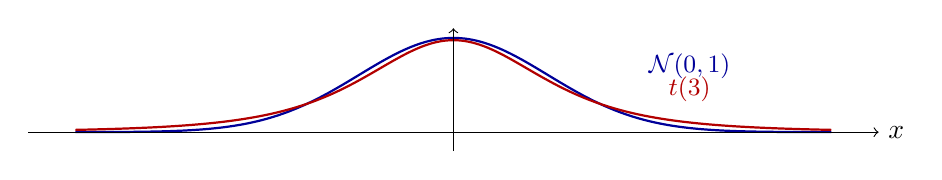
\begin{tikzpicture}[scale=1.2]
    % Normal curve
    \draw[thick, blue!60!black, domain=-4:4, samples=100, smooth]
        plot (\x, {2.5*exp(-(\x)^2/2)/sqrt(2*pi)});
    \node[blue!60!black, font=\small] at (2.5, 0.7) {$\mathcal{N}(0,1)$};
    % t with df=3 (heavier tails)
    \draw[thick, red!70!black, domain=-4:4, samples=100, smooth]
        plot (\x, {2.5*(1+(\x)^2/3)^(-2)/ (sqrt(3)*1.4826)});
    \node[red!70!black, font=\small] at (2.5, 0.45) {$t(3)$};
    \draw[->] (-4.5,0) -- (4.5,0) node[right] {$x$};
    \draw[->] (0,-0.2) -- (0,1.1);
\end{tikzpicture}
\end{center}

\subsubsection{核心桥梁：$S$ 怎样与 $\chi^2$ 挂钩——从 $t$ 定义到 $t$ 检验}

\emph{这是理解 $t$ 检验最关键的一步。} $t$ 分布的定义是 $T = \frac{X}{\sqrt{Y/n}}$，其中 $X \sim \mathcal{N}(0,1)$，$Y \sim \chi^2(n)$。
但 $t$ 检验的统计量是 $T = \frac{\bar{X} - \mu_0}{S/\sqrt{n}}$——这里 $S$ 是样本标准差，\textbf{不是} $\chi^2$ 变量。
那么 $T$ 为什么服从 $t$ 分布？

关键在于\textbf{分子分母同做代数变形}，把 $S$ 转化为 $\chi^2$ 的形式。

\medskip
\textbf{完整推导：}

\begin{enumerate}[label=\textbf{第 \arabic* 步}, leftmargin=*]

    \item \textbf{分离 $\sigma$ —— 分子分母同除 $\sigma$。}

    \begin{equation}
        T = \frac{\bar{X} - \mu_0}{S / \sqrt{n}}
          = \frac{(\bar{X} - \mu_0) / (\textcolor{blue}{\sigma} / \sqrt{n})}
                 {\sqrt{S^2 / \textcolor{blue}{\sigma}^2}}
          = \frac{Z}{\sqrt{\dfrac{(n-1)S^2 / \sigma^2}{n-1}}}.
    \end{equation}

    令：
    \begin{itemize}
        \item $Z = \dfrac{\bar{X} - \mu_0}{\sigma / \sqrt{n}}$ —— 分子是标准正态
        \item $Y = \dfrac{(n-1)S^2}{\sigma^2}$ —— 分母根号里的分子
    \end{itemize}

    \item \textbf{识别两个分量的分布。}

    \begin{itemize}
        \item $Z \sim \mathcal{N}(0,1)$：这是正态总体下样本均值的标准化形式。
        \item $Y = \dfrac{(n-1)S^2}{\sigma^2} \sim \chi^2(n-1)$：这是正态总体抽样分布的定理——\\
        已在 $\chi^2$ 节"核心问题"中完整推导。本质是 $n$ 个标准正态平方和，用 $\bar{X}$ 替代 $\mu$ 后自由度减 1。
        \item \textbf{$\bar{X}$ 与 $S^2$ 相互独立}（仅对正态总体成立！）$\implies$ $Z$ 与 $Y$ 独立。
    \end{itemize}

    \item \textbf{套入 $t$ 分布的定义。}

    \begin{equation}
        T = \frac{Z}{\sqrt{Y / (n-1)}} \sim t(n-1).
    \end{equation}

    这正是 $t$ 分布的标准形式：分子 $\mathcal{N}(0,1)$，分母 $\sqrt{\chi^2_{n-1} / (n-1)}$，两者独立。

\end{enumerate}

\medskip
\textbf{一句话总结：}

\[
\underbrace{\frac{\bar{X} - \mu_0}{S / \sqrt{n}}}_{\text{你计算的东西}}
\;=\;
\frac{
    \overbrace{\frac{\bar{X} - \mu_0}{\sigma / \sqrt{n}}}^{\sim\; \mathcal{N}(0,1)}
}{
    \sqrt{
        \underbrace{\frac{(n-1)S^2}{\sigma^2}}_{\sim\; \chi^2(n-1)}
        \Big/ (n-1)
    }
}
\;\sim\; t(n-1).
\]

\textbf{没有这两个事实，$t$ 检验就不存在：}
\begin{enumerate}[label=(\arabic*)]
    \item $\dfrac{(n-1)S^2}{\sigma^2} \sim \chi^2(n-1)$ —— 把 $S$ 桥接到 $\chi^2$
    \item $\bar{X}$ 与 $S^2$ 独立 —— 保证分子分母独立（仅正态总体有此性质）
\end{enumerate}

这就是为什么 $t$ 检验\emph{假设数据来自正态总体}——如果总体不正态，$\bar{X}$ 和 $S^2$ 不一定独立，
$(n-1)S^2/\sigma^2$ 也不精确服从 $\chi^2$，整个推导链条就断了。

\subsubsection{典型应用场景}

\begin{enumerate}[label=(\arabic*)]
    \item \textbf{小样本均值的置信区间与检验（$\sigma$ 未知）}：最核心的应用。
    如 10 个病人的血压变化是否显著？用 $t$ 检验
    \item \textbf{两样本均值比较（$t$ 检验）}：A/B 测试中判断实验组与对照组均值差异是否显著
    \item \textbf{回归系数的显著性检验}：$\frac{\hat{\beta}_j}{\mathrm{SE}(\hat{\beta}_j)} \sim t(n-p-1)$，
    判断某个特征对目标变量是否有显著影响（线性回归输出中的 $p$ 值来自 $t$ 分布）
    \item \textbf{配对 $t$ 检验}：同一样本处理前后比较，如服药前 vs. 服药后
    \item \textbf{机器学习中的特征筛选}：对每个特征做两样本 $t$ 检验，筛选出有区分力的特征
\end{enumerate}

\subsubsection{单样本 $t$ 检验——完整流程与实例}

\textbf{问题：} 某新药声称能降低收缩压。给 $n = 10$ 位患者服药，测量服药前后收缩压的差值 $X_i$
（$X_i =$ 服药后 $-$ 服药前，负值表示血压下降）：

\begin{center}
\begin{tabular}{c|cccccccccc}
\toprule
患者 & 1 & 2 & 3 & 4 & 5 & 6 & 7 & 8 & 9 & 10 \\
\midrule
血压变化 $x_i$ (mmHg) & $-5$ & $-2$ & $-8$ & $-3$ & $-1$ & $-6$ & $-4$ & $-7$ & $-2$ & $-3$ \\
\bottomrule
\end{tabular}
\end{center}

\begin{itemize}
    \item 样本量 $n = 10$
    \item 样本均值 $\bar{x} = \frac{1}{10}\sum x_i = -4.1$（平均降低 4.1 mmHg）
    \item 样本标准差 $s = \sqrt{\frac{1}{9}\sum (x_i - \bar{x})^2} \approx 2.38$
    \item 总体标准差 $\sigma$ 未知！
\end{itemize}

\textbf{第 1 步：建立假设。}

\begin{itemize}
    \item $H_0$：$\mu = 0$（药物无效，血压没有变化）
    \item $H_1$：$\mu < 0$（药物有效，血压下降）\quad ——单侧（左尾）检验
\end{itemize}

\textbf{第 2 步：构造检验统计量。}

若 $\sigma$ 已知，自然用 $Z = \frac{\bar{X} - \mu_0}{\sigma/\sqrt{n}} \sim \mathcal{N}(0,1)$。
但 $\sigma$ \emph{未知}，只能用 $S$ 替代 $\sigma$，统计量变为：

\begin{equation}
    \boxed{T = \frac{\bar{X} - \mu_0}{S / \sqrt{n}} \sim t(n-1)}.
\end{equation}

代入数值：
\begin{equation}
    t = \frac{-4.1 - 0}{2.38 / \sqrt{10}} = \frac{-4.1}{0.753} \approx -5.45.
\end{equation}

\textbf{为什么不能直接用正态分布？} 分母 $S$ 是随机变量（不是常数 $\sigma$），引入了额外的不确定性。
$t$ 分布的尾部比正态更厚，正是为了补偿"用 $S$ 替代 $\sigma$"带来的额外风险。
当 $n = 10$（$df = 9$）时，$t_{0.05}(9) \approx 1.833$ 而 $z_{0.05} = 1.645$——$t$ 检验更保守，
需要更大的 $|T|$ 才能拒绝 $H_0$。

\textbf{第 3 步：确定自由度，查临界值。}

自由度为 $n - 1 = 9$。取 $\alpha = 0.05$。

因为是单侧左尾检验：拒绝域为 $T < -t_{\alpha}(n-1)$。
查表得 $t_{0.05}(9) \approx 1.833$，故拒绝域为 $T < -1.833$。

\textbf{第 4 步：做决策。}

$t = -5.45 < -1.833$，检验统计量落入拒绝域。
\textbf{拒绝 $H_0$}，认为药物能显著降低血压。

等价地，可计算 $p$ 值：$p = P(T < -5.45 \mid df=9) \ll 0.001$，远小于 $\alpha = 0.05$。

\textbf{第 5 步：报告同时给出置信区间（良好实践）。}

不仅说"有无效果"，还应给出效果大小的范围估计。$\mu$ 的 $95\%$ 置信区间（双侧）：

\begin{equation}
    \bar{x} \;\pm\; t_{\alpha/2}(n-1) \cdot \frac{s}{\sqrt{n}}
    = -4.1 \;\pm\; t_{0.025}(9) \times 0.753.
\end{equation}

查表 $t_{0.025}(9) \approx 2.262$：
\begin{equation}
    -4.1 \;\pm\; 2.262 \times 0.753 = (-5.80,\; -2.40).
\end{equation}

\textbf{解读：} 有 95\% 的把握认为，该药平均降低收缩压 2.40 到 5.80 mmHg（整个区间在 0 以下，与拒绝 $H_0$ 的结论一致）。

\medskip
\textbf{双侧 vs. 单侧：什么时候用哪个？}

\begin{center}
\renewcommand{\arraystretch}{1.3}
\begin{tabular}{c|c|c}
\toprule
& \textbf{双侧检验} & \textbf{单侧检验} \\
\midrule
$H_1$ & $\mu \neq \mu_0$（有差异，不管方向） & $\mu < \mu_0$ 或 $\mu > \mu_0$（有方向的差异） \\
拒绝域 & $|T| > t_{\alpha/2}(n-1)$ & $T < -t_{\alpha}(n-1)$ 或 $T > t_{\alpha}(n-1)$ \\
适用场景 & 新药是否\emph{改变}了血压（不确定方向） & 新药是否\emph{降低}了血压（有先验方向） \\
\bottomrule
\end{tabular}
\end{center}

\medskip
\textbf{单样本 $t$ 检验与 $z$ 检验的对比总结：}

\begin{center}
\footnotesize
\renewcommand{\arraystretch}{1.4}
\begin{tabular}{p{2.8cm}|p{4.2cm}|p{5cm}}
\toprule
& \textbf{$z$ 检验（$\sigma$ 已知）} & \textbf{$t$ 检验（$\sigma$ 未知）} \\
\midrule
检验统计量 & $Z = \dfrac{\bar{X} - \mu_0}{\textcolor{blue}{\sigma}/\sqrt{n}}$ & $T = \dfrac{\bar{X} - \mu_0}{\textcolor{red}{S}/\sqrt{n}}$ \\
\midrule
分布 & $\mathcal{N}(0,1)$（精确） & $t(n-1)$（$\sigma$ 未知时的精确分布） \\
\midrule
适用条件 & $\sigma$ 已知，或 $n$ 很大（$\ge 30$） & $\sigma$ 未知，尤其 $n < 30$ \\
\midrule
实际中多用谁 & 几乎只存在于教科书 & \textbf{现实中的默认选择}——$\sigma$ 几乎永远是未知的 \\
\midrule
关系 & $n \to \infty$ 时 $t \to z$ & $n$ 大时 $t \approx z$，$n \ge 30$ 时差异可忽略 \\
\bottomrule
\end{tabular}
\end{center}

\subsubsection{关键前提：为什么假定 $X_i$ 服从正态分布？违背了怎么办？}

$t$ 检验的全部推导基于一个核心前提：\textbf{数据来自正态总体}。
在血压例子中，这意味着假定 10 位患者的血压变化值 $X_1,\dots,X_{10} \stackrel{\mathrm{i.i.d.}}{\sim} \mathcal{N}(\mu, \sigma^2)$。

\textbf{这并不是一个"已被证明的事实"，而是一个建模假设。}

\medskip
\textbf{为什么这个假设在血压例子中合理？}

血压是大量微小生理因素叠加的结果——心率、血管阻力、激素水平、测量误差……根据中心极限定理，
大量独立微小效应的叠加趋向正态分布。同类医学研究中，血压变化确实通常近似正态。

\textbf{但并非所有场景都适用：}

\begin{center}
\footnotesize
\renewcommand{\arraystretch}{1.3}
\begin{tabular}{c|c|c}
\toprule
\textbf{数据类型} & \textbf{为什么不正态} & \textbf{合适的方法} \\
\midrule
治愈天数 & 右偏（有下界 0，不能为负） & Wilcoxon 符号秩检验，或对数变换后做 $t$ 检验 \\
消费金额 & 长尾，少数人消费极高 & 同上 \\
点击/计数 & 泊松型（方差 $=$ 均值） & 泊松回归，或平方根变换 \\
比例/百分比 & 有界 $[0,1]$，两端堆积 & Beta 回归，或 logit 变换 \\
\bottomrule
\end{tabular}
\end{center}

\medskip
\textbf{正态假定违背了会怎样？}

$t$ 检验对正态性偏离有一定\emph{稳健性}，但并非无限制：

\begin{center}
\renewcommand{\arraystretch}{1.3}
\begin{tabular}{c|c|c}
\toprule
\textbf{偏离程度} & \textbf{后果} & \textbf{$n$ 的影响} \\
\midrule
轻度偏态（略有不对称） & $t$ 检验近似有效，影响不大 & $n$ 越大越安全（CLT 保证 $\bar{X}$ 渐近正态） \\
重尾或有离群值       & 第一类错误率膨胀，可能误拒 $H_0$ & $n$ 再大也救不了（离群值不因 $n$ 增大而消失） \\
严重偏态             & 检验功效下降，可能漏掉真实效应 & 需要换非参数方法 \\
\bottomrule
\end{tabular}
\end{center}

\medskip
\textbf{实际诊断流程（在跑 $t$ 检验之前）：}

\begin{enumerate}[label=(\arabic*)]
    \item \textbf{画 Q-Q 图}（详见下方详解）
    \item \textbf{做 Shapiro-Wilk 检验}：$H_0$ 为"数据来自正态分布"。若 $p > 0.05$，不拒绝正态性假定。
    \item \textbf{若正态性不满足且 $n$ 小}：改用 \textbf{Wilcoxon 符号秩检验}——不要求正态，只要求分布对称。\\
    这是 $t$ 检验最常用的非参数替代方案。
    \item \textbf{若 $n$ 较大（$\ge 30$）}：由 CLT，$\bar{X}$ 近似正态，$t$ 检验仍可近似使用（但仍需留意离群值）。
\end{enumerate}

\subsubsection{Q-Q 图详解：为什么能检查正态性？}

\textbf{什么是 Q-Q 图？}

Q-Q 图（Quantile-Quantile Plot，分位数-分位数图）将样本的分位数与某个理论分布（如正态）的分位数画在同一张散点图上：

\begin{itemize}
    \item \textbf{横轴}：理论分位数——例如 $\mathcal{N}(0,1)$ 的第 $1/(n+1), 2/(n+1), \dots, n/(n+1)$ 分位数
    \item \textbf{纵轴}：样本分位数——将 $n$ 个数据从小到大排序后对应的值
\end{itemize}

\textbf{为什么正态数据落在一条直线上？}

这是 Q-Q 图最核心的数学原理。

假设数据真的来自正态总体 $X \sim \mathcal{N}(\mu, \sigma^2)$。将 $X$ 标准化：$Z = (X - \mu)/\sigma \sim \mathcal{N}(0,1)$。

反过来写：$X = \mu + \sigma Z$。这意味着样本的第 $p$ 分位数 $Q_X(p)$ 与标准正态的第 $p$ 分位数 $Q_Z(p)$ 之间有\textbf{线性关系}：

\begin{equation}
    \boxed{Q_X(p) = \mu + \sigma \cdot Q_Z(p)}.
\end{equation}

因此，若以 $Q_Z(p)$ 为横轴、$Q_X(p)$ 为纵轴画散点图，正态数据应沿一条直线分布：
\begin{itemize}
    \item \textbf{截距} $\approx \mu$（数据均值）
    \item \textbf{斜率} $\approx \sigma$（数据标准差）
\end{itemize}

\emph{数据是否在一条直线上}就是 Q-Q 图判断正态性的全部依据——\textbf{形状比位置更重要}。
截距和斜率不同只说明 $\mu \neq 0$ 或 $\sigma \neq 1$，这并不违背正态性。

\medskip
\textbf{常见偏离模式及其含义：}

\begin{center}
\renewcommand{\arraystretch}{1.3}
\begin{tabular}{c|c|c}
\toprule
\textbf{Q-Q 图形状} & \textbf{说明} & \textbf{暗示的分布特征} \\
\midrule
点沿一条直线 & 正态性良好 & 数据符合正态 \\
两端向上翘（S 形上凸） & 右尾偏长 & \textbf{右偏（正偏）}，如收入数据 \\
两端向下弯（S 形下凹） & 左尾偏长 & \textbf{左偏（负偏）}，如考试高分数据 \\
左端下弯、右端上翘（反 S 形） & 两端都长 & \textbf{重尾分布}（比正态更易出极端值） \\
左端上翘、右端下弯 & 两端都短 & \textbf{轻尾分布}（如均匀分布） \\
\bottomrule
\end{tabular}
\end{center}

\begin{figure}[htbp]
\centering
\begin{tikzpicture}[scale=1.0]

% ---- Normal Q-Q (good) ----
\begin{scope}[local bounding box=good]
    \draw[->] (-2.5,0) -- (2.5,0) node[right] {\footnotesize 理论分位数};
    \draw[->] (0,-2.5) -- (0,2.5) node[above] {\footnotesize 样本分位数};
    \draw[gray!40] (-2.2,-2.2) -- (2.2,2.2);
    % points along the line with small scatter
    \foreach \x in {-2,-1.5,-1,-0.5,0,0.5,1,1.5,2} {
        \fill[blue!60!black] (\x+0.05*rand, \x+0.05*rand) circle (1.5pt);
    }
    \node[font=\small\sffamily] at (0,-2.8) {\textbf{正常（正态）}};
\end{scope}

% ---- Right-skewed ----
\begin{scope}[xshift=5.5cm, local bounding box=skew]
    \draw[->] (-2.5,0) -- (2.5,0) node[right] {\footnotesize 理论分位数};
    \draw[->] (0,-2.5) -- (0,2.5) node[above] {\footnotesize 样本分位数};
    \draw[gray!40] (-2.2,-2.2) -- (2.2,2.2);
    % S-shaped: upper end goes up
    \draw[red!70!black, thick, domain=-2.2:2.2, samples=50, smooth]
        plot (\x, {\x + 0.3*\x*\x*\x/4});
    \node[font=\small\sffamily] at (0,-2.8) {\textbf{右偏（S 形上凸）}};
\end{scope}

% ---- Heavy-tailed ----
\begin{scope}[xshift=11cm, local bounding box=heavy]
    \draw[->] (-2.5,0) -- (2.5,0) node[right] {\footnotesize 理论分位数};
    \draw[->] (0,-2.5) -- (0,2.5) node[above] {\footnotesize 样本分位数};
    \draw[gray!40] (-2.2,-2.2) -- (2.2,2.2);
    % Reverse S: left goes down, right goes up
    \draw[red!70!black, thick, domain=-2.2:2.2, samples=50, smooth]
        plot (\x, {\x - 0.25*\x*\x*\x/4});
    \node[font=\small\sffamily] at (0,-2.8) {\textbf{重尾（反 S 形）}};
\end{scope}

\end{tikzpicture}
\caption{Q-Q 图的三种典型模式。左：正态数据，点沿直线分布。中：右偏数据，右端向上翘（S 形上凸）。右：重尾数据，左端下弯、右端上翘（反 S 形）。灰色对角线为参考线 $y=x$。}
\label{fig:qqplot}
\end{figure}

\medskip
\textbf{Q-Q 图 vs. 直方图：为什么 Q-Q 图更灵敏？}

\begin{itemize}
    \item 直方图：依赖分组宽度选择，小样本时很难判断尾部形态
    \item Q-Q 图：直接比较分位数，对尾部偏离特别敏感（因为两端点稀疏，偏离一目了然），且不依赖任何参数选择
\end{itemize}

\textbf{实操规则：} 如果 Q-Q 图上的点\emph{大致}沿一条直线，不必追求完美贴合（特别是两端几个点略有波动是正常的）。
真正需要警惕的是\emph{系统性弯曲}——所有点整体呈弧形或 S 形。

\medskip
\textbf{与 Shapiro-Wilk 检验的互补关系：}

\begin{center}
\renewcommand{\arraystretch}{1.3}
\begin{tabular}{c|c|c}
\toprule
& \textbf{Q-Q 图} & \textbf{Shapiro-Wilk 检验} \\
\midrule
本质 & 可视化工具 & 统计假设检验 \\
优势 & 直观，一眼看出偏离\emph{类型}（偏态/重尾） & 给出 $p$ 值，客观判断 \\
劣势 & 依赖人眼判断，主观 & $n$ 大时过于敏感（轻微偏离也拒绝 $H_0$） \\
最佳实践 & \multicolumn{2}{c}{\textbf{两者结合}：先看 Q-Q 图判断偏离类型和程度，必要时用 SW 检验佐证} \\
\bottomrule
\end{tabular}
\end{center}

\begin{remark}[关于 CLT 的一个重要但常被忽视的细节]
CLT 保证了 $\bar{X}$ 的渐近正态性，但 $t$ 检验还需要 $S^2$ 的行为。
若总体非正态，$(n-1)S^2/\sigma^2$ 不再精确服从 $\chi^2(n-1)$，且 $\bar{X}$ 与 $S^2$ 也不一定独立。
因此 $n=30$ 的"经验法则"只能视为一个便利的近似，\emph{并非严格的数学保证}。
最安全的做法始终是用 Q-Q 图检查正态性，有疑虑时换非参数方法。
\end{remark}

\subsubsection{定义与性质}

\begin{definition}[$t$ 分布]
设 $X \sim \mathcal{N}(0,1)$，$Y \sim \chi^2(n)$，且 $X$ 与 $Y$ 相互独立，则
\begin{equation}
    T = \frac{X}{\sqrt{Y / n}} \sim t(n),
\end{equation}
称 $T$ 服从自由度为 $n$ 的\textbf{$t$ 分布}。
\end{definition}

\textbf{性质：}
\begin{itemize}
    \item PDF 关于 $x = 0$ 对称，$\E[T] = 0$（$n > 1$ 时）
    \item $\Var(T) = \dfrac{n}{n-2}$（$n > 2$）
    \item $n \to \infty$ 时 $t(n) \to \mathcal{N}(0,1)$
    \item $n = 1$ 时即为柯西分布（期望不存在，尾部极厚）
\end{itemize}

\begin{definition}[$t$ 分布的上 $\alpha$ 分位点]
点 $t_{\alpha}(n)$ 满足 $P(T > t_{\alpha}(n)) = \alpha$。
由对称性：$t_{1-\alpha}(n) = -t_{\alpha}(n)$。
\end{definition}

\subsection{$F$ 分布}

\subsubsection{历史背景}

$F$ 分布由英国统计学家 \textbf{Ronald A. Fisher}（费希尔）在 1920 年代提出，并以他姓氏的首字母命名。
Fisher 是现代统计学的奠基人之一——他提出了极大似然估计、实验设计、ANOVA 等核心方法论。
$F$ 分布最初正是为\emph{方差分析（ANOVA）}设计的。

\subsubsection{直观理解}

$F$ 分布本质上是\emph{两个独立的 $\chi^2$ 变量（各自除以自由度）的比值}：
\begin{equation}
    F = \frac{\chi^2_1 / n_1}{\chi^2_2 / n_2}.
\end{equation}

\textbf{这意味着什么？} $F$ 统计量比较两个方差（或两种变异性来源）的大小：
\begin{itemize}
    \item 分子 = "组间方差"，反映不同组之间均值的差异
    \item 分母 = "组内方差"，反映组内个体的随机波动
    \item 如果 $F \approx 1$，组间差异和组内波动差不多 → 各组可能来自同一总体
    \item 如果 $F \gg 1$，组间差异远大于随机波动 → 至少有一组明显不同
\end{itemize}

\textbf{与 $t$ 分布的关系：} $T \sim t(n)$ $\iff$ $T^2 \sim F(1, n)$。$t$ 检验（比较两组均值）是 ANOVA（比较多组均值）在 $k=2$ 时的特例。

\subsubsection{典型应用场景}

\begin{enumerate}[label=(\arabic*)]
    \item \textbf{方差分析（ANOVA）}：判断三组或以上样本的均值是否有显著差异。\\
    例：三种教学方法的效果是否不同？A/B/C 三个版本的点击率是否不同？
    \item \textbf{两正态总体方差比的检验与置信区间}：检验 $H_0: \sigma_1^2 = \sigma_2^2$。\\
    例：新工艺是否比旧工艺的波动更小（更稳定）？
    \item \textbf{回归模型的整体显著性检验（$F$ 检验）}：判断所有回归系数是否同时为 0。\\
    $F = \frac{R^2 / p}{(1-R^2)/(n-p-1)} \sim F(p, n-p-1)$，检验"模型是否比纯截距模型好"
    \item \textbf{机器学习中的特征选择}：ANOVA $F$ 检验用于评估每个数值特征与分类标签的关联强度，
    scikit-learn 中的 \verb|f_classif| 和 \verb|SelectKBest| 即基于此
    \item \textbf{模型比较}：比较两个嵌套模型的拟合优度是否有显著差异（Partial $F$ 检验）
\end{enumerate}

\subsubsection{单因素 ANOVA——完整流程与实例}

\textbf{问题：} 三种教学方法（A: 传统讲授，B: 视频自学，C: 互动讨论）是否对考试成绩有不同影响？
每种方法随机分配 6 名学生，期末考试成绩如下：

\begin{center}
\begin{tabular}{c|cccccc|c}
\toprule
\textbf{方法} & \multicolumn{6}{c|}{\textbf{学生成绩}} & \textbf{组均值} \\
\midrule
A（传统） & 78 & 82 & 85 & 90 & 76 & 88 & $\bar{x}_A = 83.17$ \\
B（视频） & 65 & 70 & 72 & 68 & 74 & 69 & $\bar{x}_B = 69.67$ \\
C（互动） & 82 & 85 & 88 & 79 & 91 & 84 & $\bar{x}_C = 84.83$ \\
\midrule
\multicolumn{7}{c}{总均值 $\bar{x} = 79.22$，总样本量 $N = 18$} \\
\bottomrule
\end{tabular}
\end{center}

\textbf{为什么不能用三次 $t$ 检验代替一次 ANOVA？}

如果做三次两两 $t$ 检验（A vs. B, B vs. C, A vs. C），每次 $\alpha = 0.05$，累积犯第一类错误的概率为
$1 - (1-0.05)^3 \approx 0.143$，远超预设的 0.05。ANOVA 通过\emph{一次检验}同时比较所有组，控制整体错误率。

\medskip
\textbf{核心直觉：比较两种"波动来源"}

把 18 个学生的成绩波动拆成两部分：

\[
\underbrace{\text{总变异 } SS_T}_{\text{18 个分数各不相同}}
\;=\;
\underbrace{\text{组间变异 } SS_B}_{\text{三组的均值不同}}
\;+\;
\underbrace{\text{组内变异 } SS_W}_{\text{同组内学生仍有差异}}
\]

\begin{itemize}
    \item 若 $H_0$ 为真（三种方法效果相同），组间差异 $\approx$ 随机波动 → $SS_B / SS_W \approx 1$
    \item 若 $H_0$ 为假（至少一种方法不同），组间差异 $\gg$ 随机波动 → $SS_B / SS_W \gg 1$
\end{itemize}

$F$ 统计量正是这两种变异的比值（经自由度调整后）。

\medskip
\textbf{第 1 步：建立假设。}

\begin{itemize}
    \item $H_0$：$\mu_A = \mu_B = \mu_C$（三种方法的总体均值相等）
    \item $H_1$：至少有一个 $\mu_i$ 不同
\end{itemize}

\textbf{第 2 步：计算各项平方和。}

\emph{总平方和} $SS_T$（Total）：每个数据点偏离总均值的平方和。

\begin{equation}
    SS_T = \sum_{i=1}^{k} \sum_{j=1}^{n_i} (x_{ij} - \bar{x})^2.
\end{equation}

\emph{组间平方和} $SS_B$（Between）：每组均值偏离总均值的平方和（按样本量加权）。

\begin{equation}
    SS_B = \sum_{i=1}^{k} n_i (\bar{x}_i - \bar{x})^2.
\end{equation}

\emph{组内平方和} $SS_W$（Within）：每个数据点偏离其组均值的平方和。

\begin{equation}
    SS_W = \sum_{i=1}^{k} \sum_{j=1}^{n_i} (x_{ij} - \bar{x}_i)^2.
\end{equation}

且恒有 $SS_T = SS_B + SS_W$（可验证）。

代入本例数值：
\begin{align}
    SS_B &= 6 \times (83.17 - 79.22)^2 + 6 \times (69.67 - 79.22)^2 + 6 \times (84.83 - 79.22)^2 \nonumber\\
         &= 6 \times (3.95^2 + (-9.56)^2 + 5.61^2) \nonumber\\
         &= 6 \times (15.60 + 91.31 + 31.47) = 830.28. \\[4pt]
    SS_W &= \sum_{\text{A}}(x - 83.17)^2 + \sum_{\text{B}}(x - 69.67)^2 + \sum_{\text{C}}(x - 84.83)^2 \nonumber\\
         &= 154.83 + 61.33 + 85.83 = 302.00. \\[4pt]
    SS_T &= 830.28 + 302.00 = 1132.28.
\end{align}

\textbf{第 3 步：计算均方（方差估计）和 $F$ 统计量。}

将平方和除以各自的自由度，得到"均方"（Mean Square）——本质上就是方差的两种估计：

\begin{equation}
    MS_B = \frac{SS_B}{k-1} = \frac{830.28}{2} = 415.14, \qquad
    MS_W = \frac{SS_W}{N-k} = \frac{302.00}{15} = 20.13.
\end{equation}

\[
\boxed{F = \frac{MS_B}{MS_W} = \frac{415.14}{20.13} = 20.62}.
\]

\textbf{自由度解释：}
\begin{itemize}
    \item $SS_B$ 的 $df = k-1 = 2$：$k$ 个组均值，受总均值一个约束
    \item $SS_W$ 的 $df = N-k = 15$：每组 $n_i$ 个数据，受各组均值 $k$ 个约束
    \item $SS_T$ 的 $df = N-1 = 17$：且 $(k-1) + (N-k) = N-1$，自由度可加
\end{itemize}

\textbf{为什么 $F$ 统计量服从 $F$ 分布？}

在 $H_0$ 和正态假定下：
\begin{itemize}
    \item $SS_B / \sigma^2 \sim \chi^2(k-1)$（组间变异，由各组均值的正态性导出）
    \item $SS_W / \sigma^2 \sim \chi^2(N-k)$（组内变异，由各组内部的正态性导出）
    \item 两者相互独立
\end{itemize}

因此：
\begin{equation}
    F = \frac{(SS_B/\sigma^2) / (k-1)}{(SS_W/\sigma^2) / (N-k)}
      = \frac{MS_B}{MS_W} \sim F(k-1,\; N-k).
\end{equation}

\textbf{第 4 步：查表，做决策。}

$df = (2, 15)$，取 $\alpha = 0.05$，查表 $F_{0.05}(2, 15) \approx 3.68$。

$F = 20.62 \gg 3.68$，\textbf{拒绝 $H_0$}——三种教学方法的效果存在显著差异。

\medskip
\textbf{第 5 步：事后两两比较（Post-hoc）。}

ANOVA 只告诉你"至少有一组不同"，但没说是哪两组。需要做\emph{事后检验}来找出具体差异。

常用方法：\textbf{Tukey HSD 检验}——在所有两两比较中控制整体错误率。

结论（示意）：A vs. B 显著（$p < 0.01$），C vs. B 显著（$p < 0.01$），A vs. C 不显著（$p > 0.05$）。
即：传统讲授和互动讨论效果相近，均显著优于视频自学。

\medskip
\textbf{ANOVA 结果的标准报告格式（APA 风格）：}

\begin{center}
\fbox{\begin{minipage}{0.85\textwidth}
\small
$F(2, 15) = 20.62,\; p < 0.001$。

三种教学方法的效果存在显著差异。Tukey HSD 事后检验表明，
传统讲授（$M = 83.17$）和互动讨论（$M = 84.83$）的考试成绩
均显著高于视频自学（$M = 69.67$），前两者之间无显著差异。
\end{minipage}}
\end{center}

\medskip
\textbf{ANOVA 的前提条件（与 $t$ 检验一致）：}

\begin{enumerate}[label=(\arabic*)]
    \item \textbf{正态性}：每组数据来自正态总体（用 Q-Q 图或 Shapiro-Wilk 检验各组）
    \item \textbf{方差齐性}：各组方差相等 $\sigma_A^2 = \sigma_B^2 = \sigma_C^2$（用 Levene 检验或 Bartlett 检验）
    \item \textbf{独立性}：观测值之间相互独立（由实验设计保证）
\end{enumerate}

\textbf{方差齐性不满足时怎么办？} 改用 Welch ANOVA（不要求等方差），原理类似 Welch $t$ 检验的推广。

\medskip
\textbf{$t$ 检验 vs. ANOVA 的关系：}

\begin{center}
\renewcommand{\arraystretch}{1.3}
\begin{tabular}{c|c|c}
\toprule
& \textbf{$t$ 检验} & \textbf{单因素 ANOVA} \\
\midrule
比较组数 & 2 组 & $k \ge 2$ 组 \\
统计量 & $T = \frac{\bar{x}_1 - \bar{x}_2}{SE}$ & $F = \frac{MS_B}{MS_W}$ \\
$k=2$ 时的关系 & $T \sim t(N-2)$ & $F \sim F(1, N-2)$，且 $T^2 = F$ \\
\bottomrule
\end{tabular}
\end{center}

\subsubsection{定义与性质}

\begin{definition}[$F$ 分布]
设 $U \sim \chi^2(n_1)$，$V \sim \chi^2(n_2)$，且 $U, V$ 相互独立，则
\begin{equation}
    F = \frac{U / n_1}{V / n_2} \sim F(n_1, n_2),
\end{equation}
称 $F$ 服从自由度为 $(n_1, n_2)$ 的\textbf{$F$ 分布}。$n_1$ 为分子（第一）自由度，$n_2$ 为分母（第二）自由度。
\end{definition}

\textbf{性质：}
\begin{equation}
    F_{1-\alpha}(n_1, n_2) = \frac{1}{F_{\alpha}(n_2, n_1)}.
\end{equation}
若 $T \sim t(n)$，则 $T^2 \sim F(1, n)$。

\subsubsection{三大抽样分布对比总结}

\begin{center}
\renewcommand{\arraystretch}{1.4}
\begin{tabular}{c|c|c|c}
\toprule
\textbf{分布} & \textbf{构造方式} & \textbf{核心用途} & \textbf{ML 中的身影} \\
\midrule
$\chi^2(n)$
    & $n$ 个独立 $\mathcal{N}(0,1)$ 的平方和
    & 方差估计、拟合优度、独立性检验
    & $\chi^2$ 特征选择、决策树 $\chi^2$ 剪枝 \\
\midrule
$t(n)$
    & $\dfrac{\mathcal{N}(0,1)}{\sqrt{\chi^2(n)/n}}$
    & 小样本均值推断、回归系数显著性
    & $t$ 检验特征筛选、A/B 测试 \\
\midrule
$F(n_1,n_2)$
    & $\dfrac{\chi^2(n_1)/n_1}{\chi^2(n_2)/n_2}$
    & 方差比较、ANOVA、模型显著性
    & ANOVA 特征选择、模型 $F$ 检验 \\
\bottomrule
\end{tabular}
\end{center}

\subsubsection{常见理解误区：各分布的适用范围被窄化了}

初学者常把三个分布和理解场景做一一映射，但实际它们的适用范围远比直觉广。

\medskip
\textbf{误区一："$\chi^2$ 只能看观测频数和期望频数的差异"}

$\chi^2$ 分布的本质是\textbf{标准正态随机变量的平方和}——频数比较只是其应用之一。
因为任何被标准化后的偏差平方累加都可能涉及 $\chi^2$，它在完全不同类型的场景中都会出现：

\begin{center}
\footnotesize
\renewcommand{\arraystretch}{1.4}
\begin{tabular}{c|c|c}
\toprule
\textbf{应用} & \textbf{数学形式} & \textbf{是"频数比较"吗？} \\
\midrule
拟合优度 / 独立性检验 & $\sum \frac{(O_i - E_i)^2}{E_i} \sim \chi^2$ & \checkmark \; 是 \\
\textbf{连续数据的方差估计} & $\frac{(n-1)S^2}{\sigma^2} \sim \chi^2(n-1)$ & $\times$\; 否——这是连续量，与频数无关 \\
$t$ 分布的底层构件 & $t = \frac{\mathcal{N}(0,1)}{\sqrt{\chi^2/df}}$ & $\times$\; 否——$\chi^2$ 在此承载方差信息 \\
$F$ 分布的底层构件 & $F = \frac{\chi^2_1/df_1}{\chi^2_2/df_2}$ & $\times$\; 否 \\
似然比检验（模型比较） & $2(\ln L_1 - \ln L_0) \xrightarrow{d} \chi^2$ & $\times$\; 否——比较两个模型的拟合优度 \\
\bottomrule
\end{tabular}
\end{center}

\medskip
\textbf{误区二："$t$ 分布只能检验 $\mu$ 是否差异显著"}

$t$ 分布的数学形式是 $T = \frac{\text{估计量} \;-\; \text{假设值}}{\text{该估计量的标准误}}$。
\textbf{只要你的统计量长成"估计值除以它的标准误"，大概率就服从 $t$ 分布}——被估计的对象不一定是 $\mu$。

\begin{center}
\footnotesize
\renewcommand{\arraystretch}{1.4}
\begin{tabular}{c|c|c}
\toprule
\textbf{应用} & \textbf{检验对象} & \textbf{是"检验 $\mu$"吗？} \\
\midrule
单样本 $t$ 检验 & 总体均值 $\mu$ & \checkmark \; 是 \\
两样本 $t$ 检验 & 两个总体均值差 $\mu_1 - \mu_2$ & \checkmark \; 是 \\
配对 $t$ 检验 & 配对差值的均值 & \checkmark \; 是 \\
\textbf{回归系数显著性} & $\beta_j = 0$？ & $\times$\; 否——这是斜率，不是均值！ \\
\textbf{相关系数检验} & $\rho = 0$？ & $\times$\; 否 \\
\textbf{两个回归系数比较} & $\beta_1 = \beta_2$？ & $\times$\; 否 \\
A/B 测试转化率 & 比例差异 & \checkmark \; 实质是两样本均值的变体 \\
\bottomrule
\end{tabular}
\end{center}

回归系数检验是 $t$ 分布\textbf{在实际工作中最高频的应用}——
`statsmodels` / R 的 `summary()` 输出里每一行的 `t value` 和 `Pr(>|t|)`，全部是 $t$ 检验。

\medskip
\textbf{三个分布的正确理解——层次关系：}

\[
\boxed{\chi^2 \;\text{是砖块}\; \longrightarrow \;
       t = \frac{\mathcal{N}(0,1)}{\sqrt{\chi^2/df}},\;
       F = \frac{\chi^2_1/df_1}{\chi^2_2/df_2}
       \;\text{是它垒出的两种建筑}}
\]

\begin{center}
\renewcommand{\arraystretch}{1.5}
\begin{tabular}{c|c|c}
\toprule
\textbf{分布} & \textbf{数学本质} & \textbf{不要窄化为} \\
\midrule
$\chi^2$ & 标准正态平方和的分布 & "只能比较频数" \\
$t$     & $\mathcal{N}(0,1) \big/ \sqrt{\chi^2/df}$ & "只能检验 $\mu$" \\
$F$     & $(\chi^2_1/df_1) \big/ (\chi^2_2/df_2)$ & "只能做 ANOVA" \\
\bottomrule
\end{tabular}
\end{center}

理解了这个层次关系，每个分布的适用范围自然就打开了——\textbf{凡是你对某个量做了标准化再平方求和，$\chi^2$ 就会出现；
凡是某个估计量除以它的标准误，$t$ 就会出现。}

\subsection{正态总体的抽样分布定理（核心定理）}

\begin{theorem}[单个正态总体]
设 $X_1, X_2, \dots, X_n$ 是来自正态总体 $\mathcal{N}(\mu, \sigma^2)$ 的样本，$\bar{X}$ 与 $S^2$ 分别为样本均值与样本方差，则：
\begin{enumerate}[label=(\arabic*)]
    \item $\bar{X} \sim \mathcal{N}\!\left(\mu,\; \dfrac{\sigma^2}{n}\right)$，
          即 $\dfrac{\bar{X} - \mu}{\sigma / \sqrt{n}} \sim \mathcal{N}(0,1)$；
    \item $\dfrac{(n-1)S^2}{\sigma^2} \sim \chi^2(n-1)$；
    \item $\bar{X}$ 与 $S^2$ \textbf{相互独立}；
    \item $\dfrac{\bar{X} - \mu}{S / \sqrt{n}} \sim t(n-1)$。
\end{enumerate}
\end{theorem}

\begin{theorem}[两个正态总体]
设 $X_1,\dots,X_{n_1} \stackrel{\mathrm{i.i.d.}}{\sim} \mathcal{N}(\mu_1, \sigma_1^2)$，
$Y_1,\dots,Y_{n_2} \stackrel{\mathrm{i.i.d.}}{\sim} \mathcal{N}(\mu_2, \sigma_2^2)$，两样本独立，则：
\begin{enumerate}[label=(\arabic*)]
    \item $\dfrac{(\bar{X} - \bar{Y}) - (\mu_1 - \mu_2)}{\sqrt{\frac{\sigma_1^2}{n_1} + \frac{\sigma_2^2}{n_2}}} \sim \mathcal{N}(0,1)$；
    \item 当 $\sigma_1^2 = \sigma_2^2 = \sigma^2$ 时，
          $\dfrac{(\bar{X} - \bar{Y}) - (\mu_1 - \mu_2)}{S_w \sqrt{\frac{1}{n_1} + \frac{1}{n_2}}} \sim t(n_1+n_2-2)$，
          其中 $S_w^2 = \dfrac{(n_1-1)S_1^2 + (n_2-1)S_2^2}{n_1+n_2-2}$；
    \item $\dfrac{S_1^2 / \sigma_1^2}{S_2^2 / \sigma_2^2} \sim F(n_1-1,\; n_2-1)$。
\end{enumerate}
\end{theorem}

% ============================================================
